% Name  
单词查找树

% Legend
在进行文法分析的时候,通常需要检测一个单词是否在我们的单词列表里。为了提高查找和定位的速度,通常都要画出与单词列表所对应的单词查找树,其特点如下:

\begin{itemize}
    \item 根节点不包含字母,除根节点外每一个节点都仅包含一个大写英文字母;
    \item 从根节点到某一节点,路径上经过的字母依次连起来所构成的字母序列,称为该节点对应的单词。单词列表中的每个词,都是该单词查找树某个节点所对应的单词;
    \item 在满足上述条件下,该单词查找树的节点数最少。
\end{itemize}

例:图一的单词列表对应图二的单词查找树

\begin{center}
    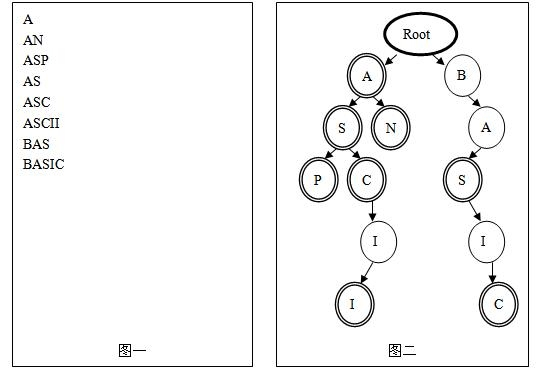
\includegraphics[bb=0 0 543 377]{trie.jpeg}
\end{center}

对一个确定的单词列表,请统计对应的单词查找树的节点数(包括根节点)。

% Input format
输入包含多行,每行一个单词。每个单词仅由大写的英文字母组成,长度不超过 $63$ 个字符。文件总长度不超过 32K,至少有一行数据。

% Output format
输出仅包含一个整数,表示单词列表对应的单词查找树的节点数。